\chapter{SGSEAM Evaluation}
\label{cha:ExperimentalDesign}

This chapter describes the experimental design for two assessment tasks: (1) applying the SGSEAM described in \autoref{cha:framework-description} to the Makahiki system described in \autoref{cha:system-description}, (2) applying the SGSEAM to a second IT infrastructure for serious games for sustainability. The goals of these assessments are: (a) obtain insights about
 the strength and weakness of the Makahiki serious game framework we designed and implemented,
 (b) obtain insights about the strength and weakness of the SGSEAM.

\section{Makahiki Assessment Overview}
The design of assessment of Makahiki using SGSEAM are two folds: (1) case studies of Makahiki instances in real-world, namely the three Kukui Cup serious games deployed in University of Hawaii at Manoa, Hawaii Pacific University, and East West Center of Hawaii. (2) in-lab experiment of assessing Makahiki system by the students taking the serious game development course in the University of Hawaii at Manoa.

\subsection{Real-world Makahiki Instances Case Studies}

Using the Makahiki as the IT infrastructure, the first and second Kukui Cup Energy challenge of University of Hawaii was held in 2011 and 2012 for over 1,000 first year students living in the residence halls. Hawaii Pacific University (HPU) held a Kukui Cup Energy challenge in Fall 2012 for about 200 students. An international organization called the East-West Center (EWC) held a Kukui Cup Energy and Water challenge for the international residents living in the residenct halls without smart meters, so the resource consumption data had to be entered by the game mangers manually.

The successful creation of serious game challenges by three different organizations provides evidence that the Makahiki serious game engine can be tailored to the differing needs of separate organizations. First, UH uses smart meters by Electro-Industries Inc., while HPU uses smart meters by EGauge Inc., and EWC collected their energy data manually. Second, while UH and HPU challenges involved only energy consumption data, the EWC challenge involved both energy and water consumption data (which was also collected manually).  Third, the IT infrastructure at UH and HPU provided authentication services using CAS and LDAP, while EWC used the built-in Django authentication. Fourth, the user interface was customized to ``brand'' each challenge with the logo, thematic elements, and the education contents of the sponsoring organizations.

\subsection{In-lab Makahiki Experiment Case Studies}

In Spring 2012, Professor Philip Johnson at the Information and Computer Science Department of University of Hawaii used Makahiki to teach a course in serious game development. The students are seniors or graduate students majored in the computer science related fields. During the course, the students will install Makahiki, configure and design a serious game instance with Makahiki, and finally develop an enhancement to the Makahiki system.

I plan to ask these students to voluntarily participate in the assessment experiments of Makahiki, in the aspects of system admin efficiency, game designer efficiency and developer efficiency. This is considered as an in-lab experiment since they are evaluating Makahiki in a class setting and using Makahiki in the development environments.

\section{Makahiki Assessment}
This section describes in details the application of SGSEAM to assess Makahiki using the settings described above.

\subsection{Player assessment}

I plan to apply the SGSEAM player assessment mechanism to the 2011 real-world Kukui Cup instance at the University of Hawaii at Manoa to study the player's experience with the Makahiki framework. There are over 1000 eligible players for this instances. They are the first year college student living in four similar structured resident halls in close vicinity. The challenge lasted for 3 weeks. Makahiki system recorded detailed logging data from every interaction between the players and the website.

To assess the effectiveness of the framework for designing games that improve player literacy in sustainability, we
conducted two energy literacy surveys, one before the challenge (pre-game) and one after
the challenge (post-game). SurveyGizimo is used to create the surveys which consists of the set of sustainability literacy and behavior questionnaires. The response from the two surveys are analyzed to provide insights about the player's literacy and behavior change.

To assess the effectiveness of the framework for designing games that produce positive change in sustainability
behaviors, we recorded and analyzed energy consumption data before, during and after the
challenge.  Before the challenge, an energy usage baseline was established. The energy consumption data is examined to understand any usage pattern or reduction during and after the challenge.

To assess the usability of the game produced by the Makahiki framework, we conducted the in-game usability survey. The survey asked the questions about the players' experience about the user interface of the game. The response from the survey is analyzed to provide insights about the game usability.

In addition to the surveys and energy data measurement, the following engagement metrics will be calculated based on the log data to assess the engagement level of the instance:

\begin{itemize}
\item active participation rate
\item number of players per day
\item average session time
\item submissions per day
\item level of social engagement
\item website errors
\end{itemize}

\subsection{System admin assessment}

There are two approaches described in SGSEAM to assess the game designer's experience: One is the experimental case study that uses the in-lab experiments, another is the interview of the system admin of a real world instance.

In the in-lab experiments, the students in the ICS691 Spring 2013 class were tasked with installing the Makahiki system into their local computers as well as the cloud environment. In order to understand how much time it takes to install the Makahiki and what problems might be encountered, I design a Google form which details the steps of installing Makahiki both locally and in the cloud, and for each step, I ask the students to record the time they spent and the problems they encountered.

Figure \ref{fig:developer-eval-form} illustrates a partial google form used for Makahiki system admin assessment. \autoref{app:googleform} includes the complete google form.
\begin{figure}[ht!]
   \centering
   \includegraphics[height=30em,width=30em]{developer-eval-form.eps}
   \caption{Makahiki Developer assessment Form}
   \label{fig:developer-eval-form}
\end{figure}

The students were also asked to provide feedback about their installation experiences in the form of blog post. In the blog post, I ask them to discuss the following topics:
\begin{itemize}
\item What is the most difficult step during installation?
\item What problems did you encounter during the installation?
\item Have you install any database, web server or similar server products prior to this assignment? Are those installations for development or production purpose?
\item If you have experience installing other servers before, How does your prior experience of installing other servers compare to the installation of Makahiki?
\item What could be improved about the Makahiki installation process?
\item Compare your experience of installing Makahiki in Heroku with installing it locally,
\end{itemize}

The qualitative data collected from the google form response and the blog post from the students will be analyzed to gain insights into how easy it is to install Makahiki, and what contributes to the efficiency of the installation.

In order to gain insights on the experience of a real world system admin who uses the Makahiki, I plan to perform interviews to the system admins of the 2013 Hawaii Pacific University (HPU) challenges.

I will analyze qualitative data collected from the interviews and email changes. The data include:
\begin{itemize}
 \item time taken to install the Makahiki
 \item time taken to maintain the Makahiki, such as backup, monitoring
 \item problems encountered
\end{itemize}

\subsection{Game designer assessment}

There are also two approaches described in SGSEAM to assess the game designer's experience: One is the experimental case study that uses the in-lab experiments, another is the interview of the game designer of a real world instance.

The students in the in-lab experiments were tasked to design a Kukui Cup like serious game using Makahiki. I designed another google form to ask students to follow the designing steps and record their time and problem encountered during their designing process. \autoref{app:googleform} has the complete google form for the steps the students need to follow.

The students were asked to provide feedback about their installation experiences in the form of blog post to discuss the following topics:
\begin{itemize}
\item What is the most difficult step during Challenge Design?
\item What problems did you encounter while designed the challenge?
\item What problems did you encounter while managing the challenge?
\item What could be improved for the Makahiki Challenge Design process?
\item What could be improved for the Makahiki Challenge Management process?
\end{itemize}

I plan to perform interviews to the real world game designers of the 2013 Hawaii Pacific University challenges. We will ask him about his game designing experiences using the Makahiki admin
 interface.

I will analyze both the qualitative data collected from the interviews and email changes with the game designers, and the quantitative collected from the admin interface log data. The qualitative data includes:
\begin{itemize}
    \item How much time did you spend to configure the challenge global settings?
    \item how much time did you spend to setup the player data?
    \item how much time did you spend to design the individual games?
    \item What problem did you encountered?
    \item Did you find it difficult to configure? what is difficult?
    \item Did you find it difficult to design a specific game? which one, what is difficult?
    \item What did you like the least when using the system?
\end{itemize}

The quantitative data includes:
\begin{itemize}
 \item time taken to configure the challenge with regarding to different designing tasks
 \item problems encountered in the log file
\end{itemize}

\subsection{Game manager assessment}
I plan to perform interviews to the real world game managers of the 2013 Hawaii Pacific University challenges to study the experience of the game management using Makahiki.

I will analyze both the qualitative data collected from the interviews and email changes with the game managers, and the quantitative collected from the admin interface log data. The qualitative data includes:
\begin{itemize}
\item How much time did you spend to approving the action submissions?
\item How much time did you spend to monitoring the game status?
\item How much time did you spend to notifying prize winners?
\item What problem did you encountered?
\item Did you find it difficult to manage? what is difficult?
\item What did you like the least when using the system?
\end{itemize}

The quantitative data include:
\begin{itemize}
 \item time taken to manage the challenge with regarding to different managing tasks
 \item problems encountered in the log file
\end{itemize}

\subsection{Developer assessment}

The students in the in-lab experiment are tasked with developing an enhancement to the Makahiki instance. This involves setting up the development environment, following the tutorial to create the "Hello world" widget using Makahiki, and finally, develop the enhancement which extends the functionality of the Makahiki system.

The students are asked to submit their development source code to the public source code repository (Github) and write a blog post to discuss their efforts to complete the development activity.

I will review their source code to compare their code to the reference implementation, analyze the blog post from the students, as well as any email correspondence from students discussing  problems during the development.

\subsection{Preliminary Results}

At the time of the writing of this proposal, I had completed some of the assessments of Makahiki using SGSEAM. The following \autoref{fig:assessment-overview} provides the overview of the status of completed work and the proposed work for applying SGSEAM to Makahiki.

\begin{figure}[ht!]
  \centering
  \begin{tabular}{|c|c|c|c|}
    \hline
    \multicolumn{1}{|p{0.2\columnwidth}|}{\centering\tabhead{Stakeholder}} &
    \multicolumn{1}{|p{0.3\columnwidth}|}{\centering\tabhead{Assessment}} &
    \multicolumn{1}{|p{0.2\columnwidth}|}{\centering\tabhead{Completed}} &
    \multicolumn{1}{|p{0.2\columnwidth}|}{\centering\tabhead{Proposed work}} \\
    \hline
    \multicolumn{1}{|p{0.2\columnwidth}|}{Players} &
    \multicolumn{1}{|p{0.3\columnwidth}|}{pre-post effectiveness experimental study} &
    \multicolumn{1}{|p{0.2\columnwidth}|}{UH 2011} &
    \multicolumn{1}{|p{0.2\columnwidth}|}{} \\
    \hline
    \multicolumn{1}{|p{0.2\columnwidth}|}{Players} &
    \multicolumn{1}{|p{0.3\columnwidth}|}{in-game usability survey} &
    \multicolumn{1}{|p{0.2\columnwidth}|}{UH 2011} &
    \multicolumn{1}{|p{0.2\columnwidth}|}{} \\
    \hline
    \multicolumn{1}{|p{0.2\columnwidth}|}{Players} &
    \multicolumn{1}{|p{0.3\columnwidth}|}{engagement metrics} &
    \multicolumn{1}{|p{0.2\columnwidth}|}{UH 2011} &
    \multicolumn{1}{|p{0.2\columnwidth}|}{} \\
    \hline
    \multicolumn{1}{|p{0.2\columnwidth}|}{System admins} &
    \multicolumn{1}{|p{0.3\columnwidth}|}{in-lab experiment case study} &
    \multicolumn{1}{|p{0.2\columnwidth}|}{ICS691} &
    \multicolumn{1}{|p{0.2\columnwidth}|}{} \\
    \hline
    \multicolumn{1}{|p{0.2\columnwidth}|}{System admins} &
    \multicolumn{1}{|p{0.3\columnwidth}|}{real-world instance case study} &
    \multicolumn{1}{|p{0.2\columnwidth}|}{} &
    \multicolumn{1}{|p{0.2\columnwidth}|}{HPU 2013} \\
    \hline
    \multicolumn{1}{|p{0.2\columnwidth}|}{Game designers} &
    \multicolumn{1}{|p{0.3\columnwidth}|}{in-lab experiment case study} &
    \multicolumn{1}{|p{0.2\columnwidth}|}{ICS691} &
    \multicolumn{1}{|p{0.2\columnwidth}|}{} \\
    \hline
    \multicolumn{1}{|p{0.2\columnwidth}|}{Game designers} &
    \multicolumn{1}{|p{0.3\columnwidth}|}{real-world instance case study} &
    \multicolumn{1}{|p{0.2\columnwidth}|}{} &
    \multicolumn{1}{|p{0.2\columnwidth}|}{HPU 2013} \\
    \hline
    \multicolumn{1}{|p{0.2\columnwidth}|}{Game managers} &
    \multicolumn{1}{|p{0.3\columnwidth}|}{real-world instance case study} &
    \multicolumn{1}{|p{0.2\columnwidth}|}{} &
    \multicolumn{1}{|p{0.2\columnwidth}|}{HPU 2013} \\
    \hline
    \multicolumn{1}{|p{0.2\columnwidth}|}{Developers} &
    \multicolumn{1}{|p{0.3\columnwidth}|}{in-lab experiment case study} &
    \multicolumn{1}{|p{0.2\columnwidth}|}{ICS691} &
    \multicolumn{1}{|p{0.2\columnwidth}|}{} \\
    \hline
    \multicolumn{1}{|p{0.2\columnwidth}|}{Developers} &
    \multicolumn{1}{|p{0.3\columnwidth}|}{internal developer case study} &
    \multicolumn{1}{|p{0.2\columnwidth}|}{} &
    \multicolumn{1}{|p{0.2\columnwidth}|}{New game development for UH2013} \\
    \hline
  \end{tabular}
  \caption{Status of Makahiki assessment}
  \label{fig:assessment-overview}
\end{figure}


\autoref{app:makahiki-assessment-report} describes the results of the completed assessments of applying SGSEAM to Makahiki.

\section{Lucid Design Dashboard assessment case study}
